\documentclass{article}
\usepackage[spanish]{babel}
\usepackage[utf8]{inputenc}
\usepackage[T1]{fontenc}
\usepackage{hyperref}
\usepackage{xcolor}
\usepackage{listings}
\usepackage{minted}
\usepackage{graphicx}
\hypersetup{
    colorlinks,
    linkcolor={red!50!black},
    citecolor={blue!50!black},
    urlcolor={blue!80!black}
}

\title{P1: Desarrollo de una Web}
\author{Daniel Ramos}
\date{\today}

\begin{document}

\maketitle

\begin{center}
    \large Herramientas HTML y CSS I
\end{center}

\newpage

\tableofcontents

\newpage

\section*{Introducción}
En esta práctica, aprenderemos a configurar el entorno de desarrollo necesario para trabajar con HTML y CSS. Esto incluye la instalación de editores de texto, navegadores web y otras herramientas útiles.

\newpage

\section{Configurando el Entorno de Desarrollo}\label{sec:configurando-el-entorno-de-desarrollo}

\subsection{Inicialización de Parcel}\label{subsec:inicializacion-de-parcel}

El primer paso ha sido inicializar el repositorio en el que se hará el desarrollo de la práctica con \lstinline|git init| y \lstinline|npm init|.

Siguiendo la guía de la web de parcel, lo siguiente ha sido instalar Parcel como dependencia del proyecto con \lstinline|npm install --save-dev parcel|.

Una vez instalado Parcel, se ha probado su correcto funcionamiento creando un \textit{Hello World}. Una vez creado el fichero \lstinline|src/index.html| se ha ejecutado el comando \lstinline|npx parcel src/index.html| y se ha comprobado que la página web de abría correctamente en el navegador como se ve en la Figura~\ref{fig:hello-world}.

 \begin{figure}[h!]
     \centering
     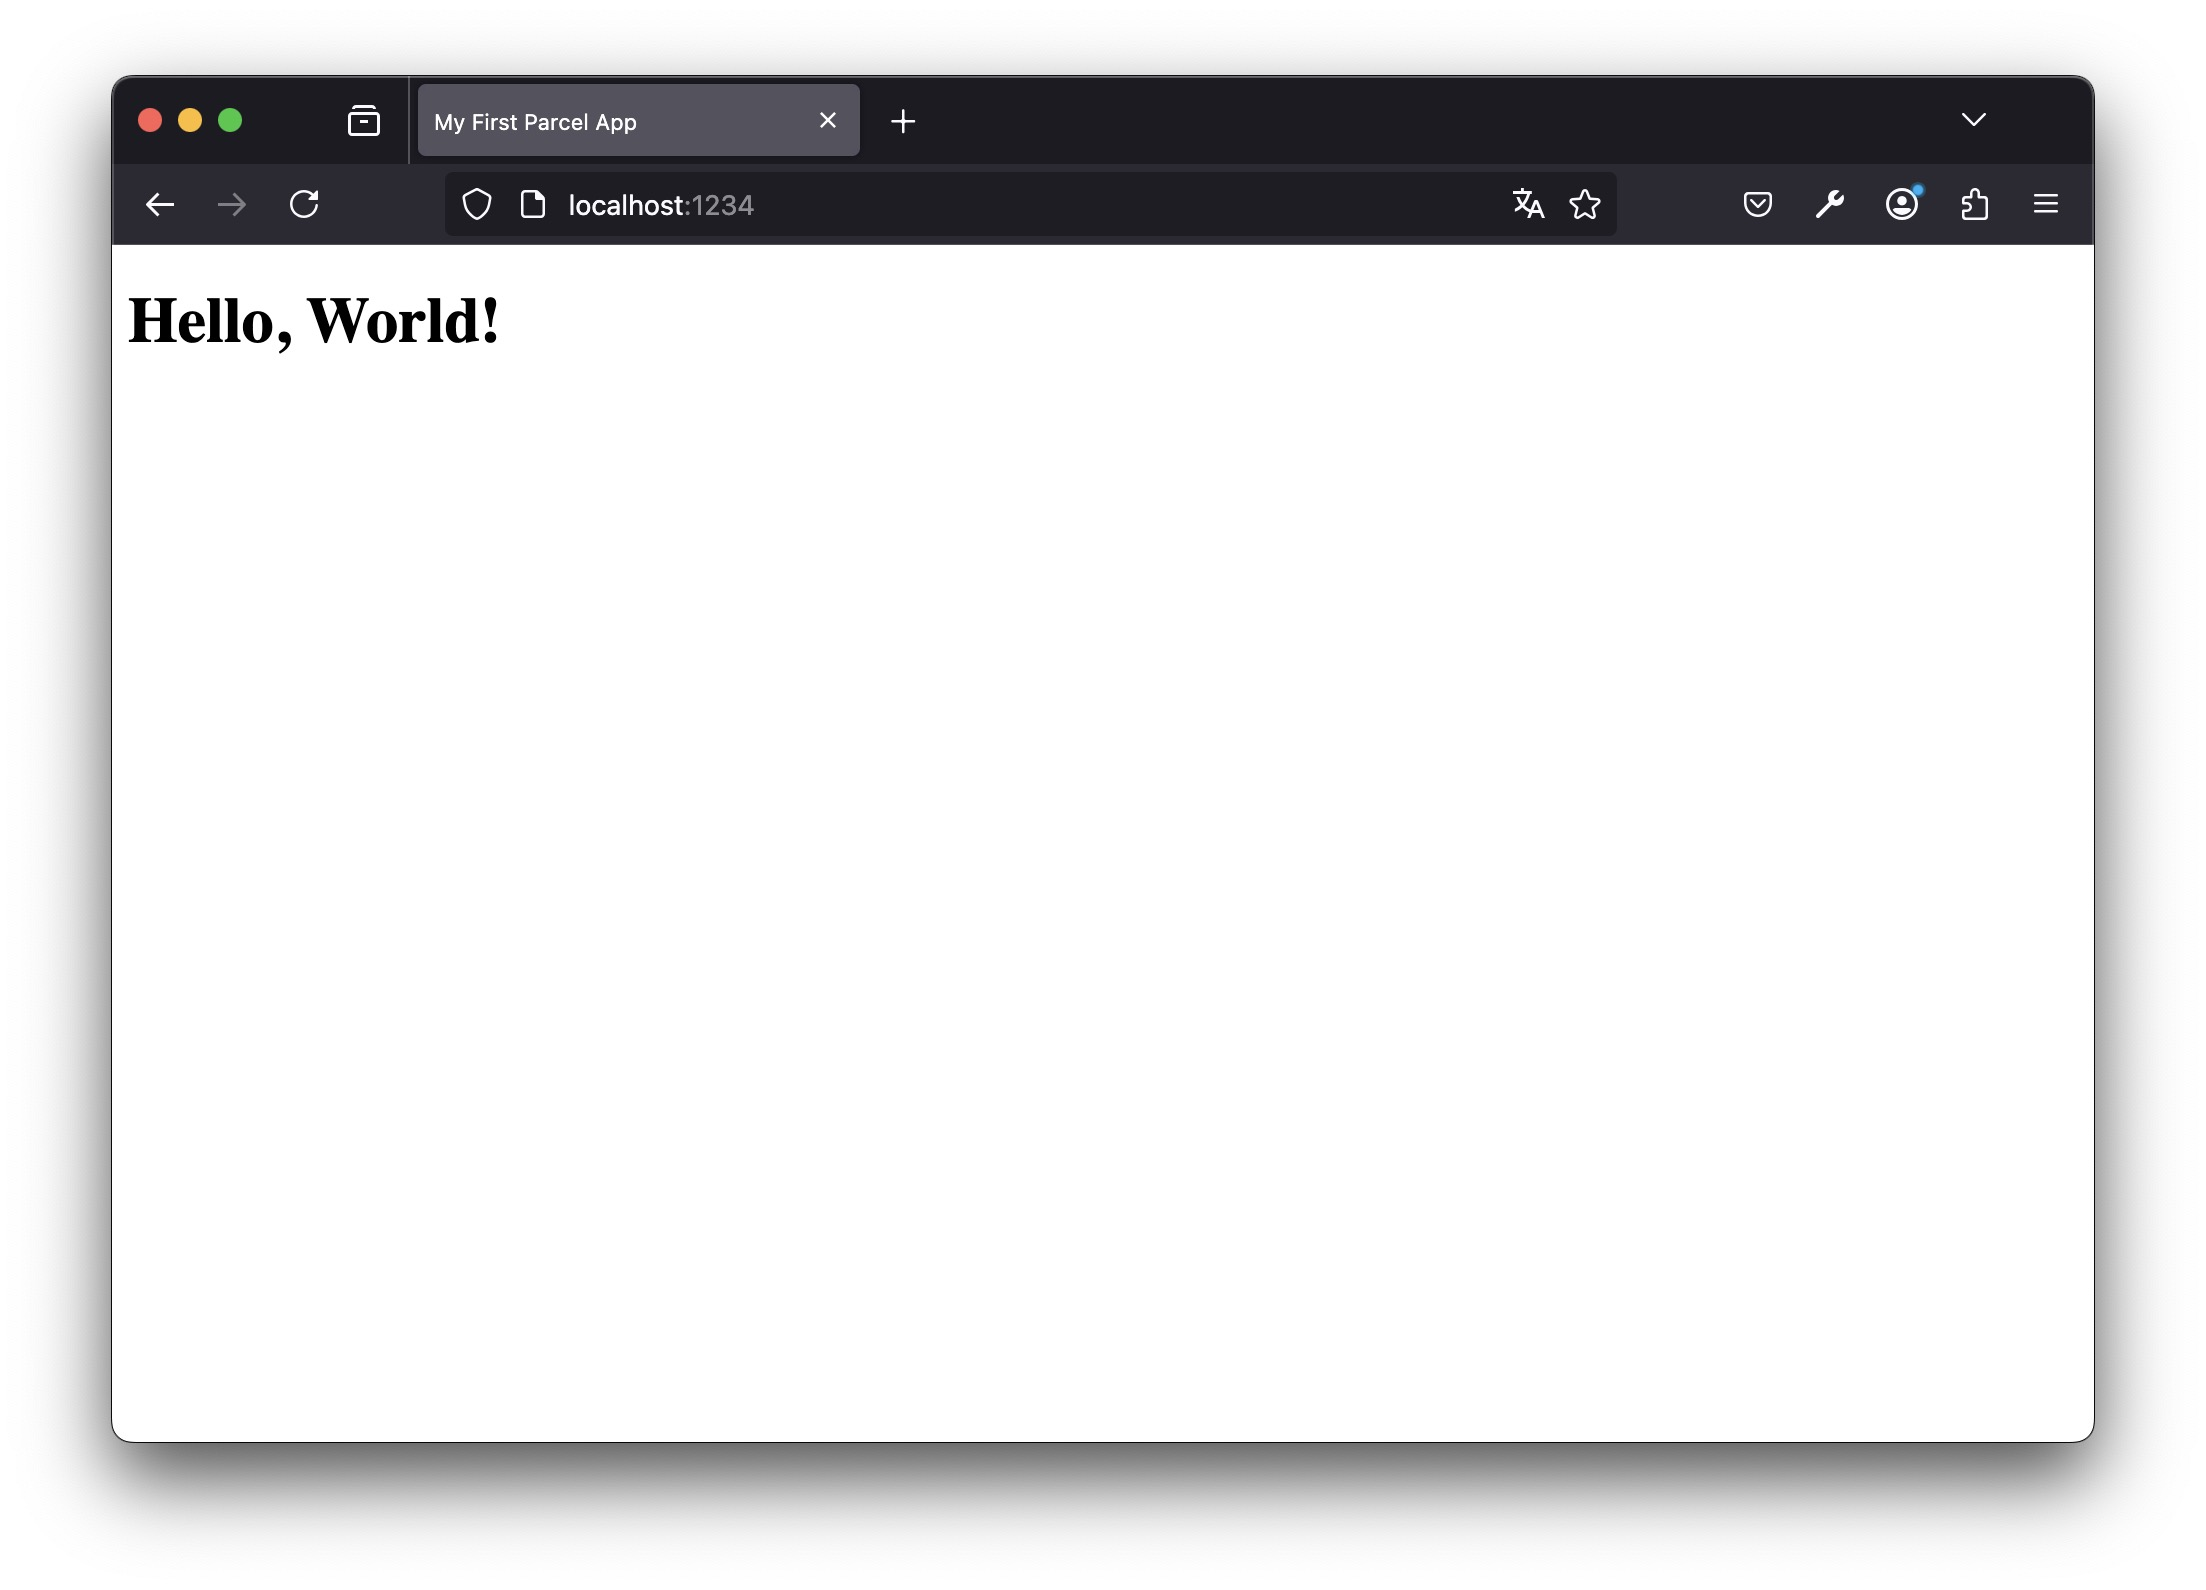
\includegraphics[width=0.8\textwidth]{./img/hello-world}
     \caption{Captura de pantalla de un Hello World básico en HTML}
     \label{fig:hello-world}
 \end{figure}

Se han realizado las modificaciones necesarias para incluir una hoja de estilos y script de ejemplos para comprobar que Parcel las procesa correctamente.
Sin tener que refrescar el navegador, los cambios se han reflejado instantáneamente en la página web (ver Figura~\ref{fig:parcel}).

 \begin{figure}[h!]
     \centering
     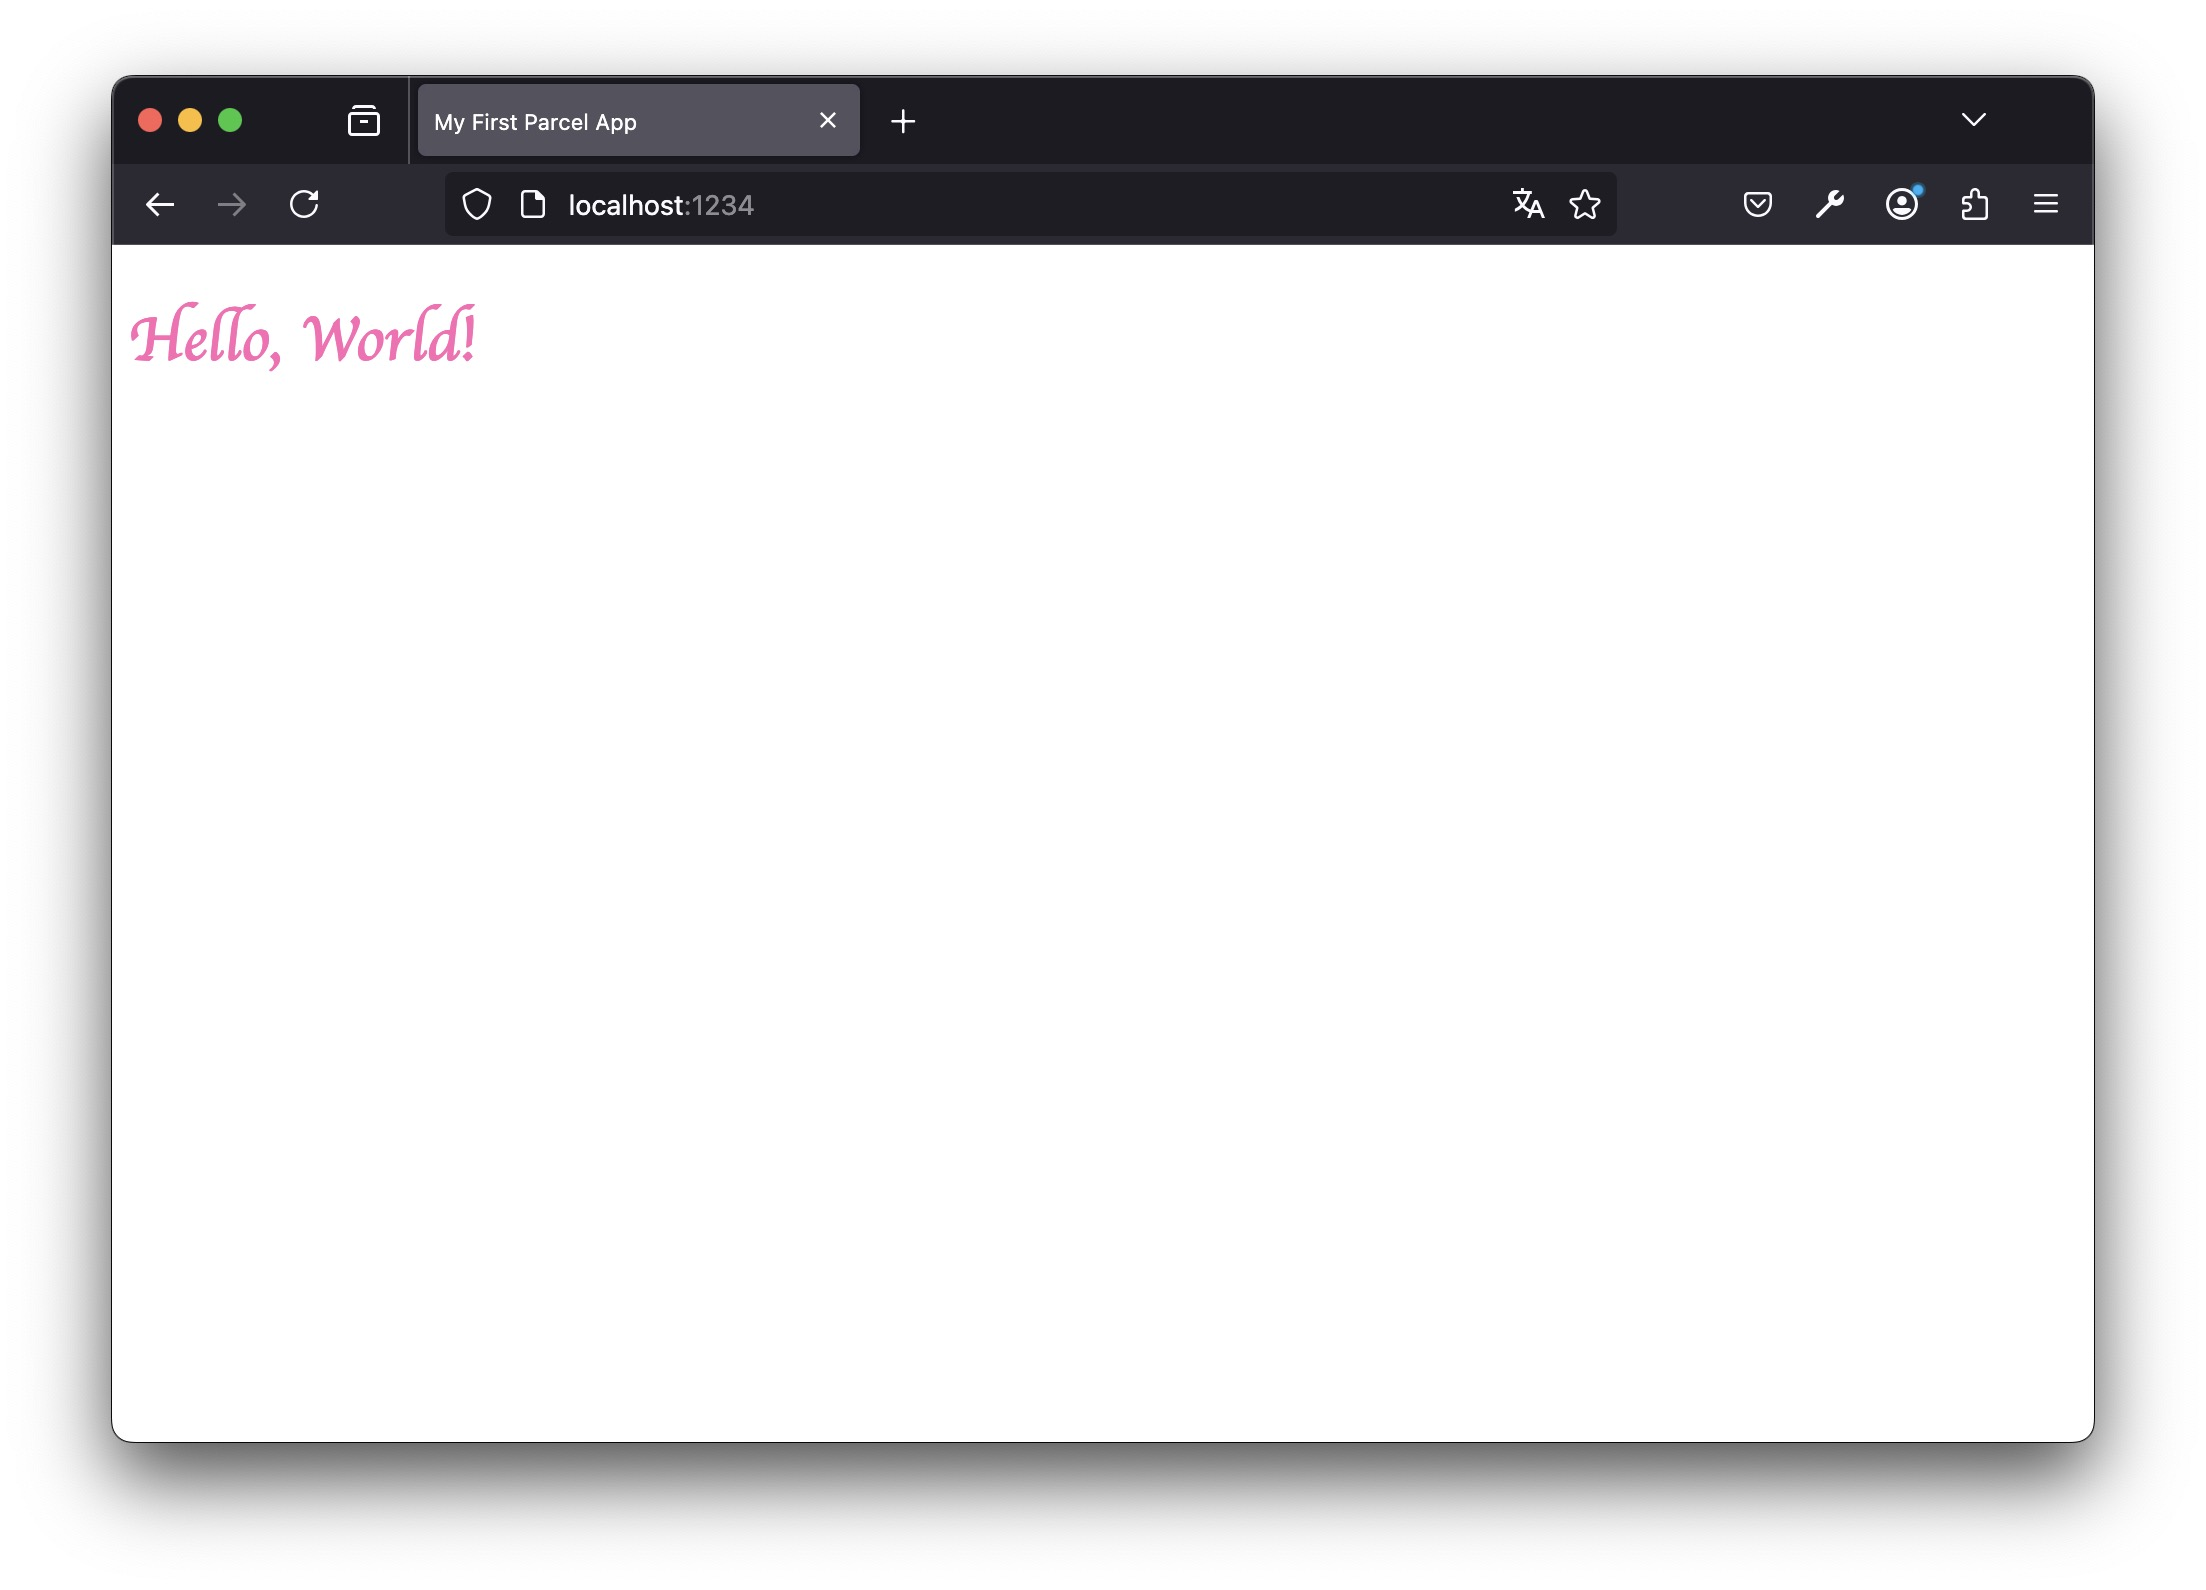
\includegraphics[width=0.8\textwidth]{./img/hello-world-styled}
     \caption{Captura de pantalla de la página web con Parcel}
     \label{fig:parcel}
 \end{figure}

Por último, siguiendo la guía, se han ajustado los scripts de \lstinline|package.json| para que sea más fácil ejecutar Parcel.
Ahora, en lugar de tener que escribir \lstinline|npx parcel src/index.html|, se puede ejecutar \lstinline|npm run start| para iniciar el servidor de desarrollo, y \lstinline|npm run build| para compilar el proyecto para producción.

Siguiendo con el enunciado del Módulo 2, se han ajustado una última vez los scripts del \lstinline|package.json|.
Se han añadido modificaciones para que se limpien los directorios de caché y de producción antes de cada compilación tal y como se puede ver en la Figura \ref{fig:package-json}.

\begin{figure}[h!]
\begin{minted}{json}
{
  "name": "hhyc-dramosac",
  "source": "src/index.html",
  "scripts": {
    "parcel:dev": "parcel",
    "parcel:build": "parcel build",
    "clean": "rimraf dist .parcel-cache",
    "start": "npm-run-all clean parcel:dev",
    "build": "npm-run-all clean parcel:build",
    "build:docs": "tectonic -Z shell-escape docs/p1.tex"
  },
  "author": "Daniel Ramos Acosta",
  "license": "ISC",
  "devDependencies": {
    "npm-run-all": "^4.1.5",
    "parcel": "^2.13.3",
    "rimraf": "^6.0.1"
  }
}
\end{minted}
\caption{Versión final del \lstinline{package.json}}
\label{fig:package-json}
\end{figure}

\subsection{Configuración de Pre y Post Procesadores}\label{subsec:configuracion-de-pre-y-post-procesadores}

El siguiente paso ha sido ajustar la configuración de \lstinline|browserslist| tal y como se propone en la documentación.
Luego, se ha ajustado para que el bundle final generado sea compatible con navegadores desde 2011.
Esta configuración probablemente sea demasiado agresiva, ya que muchos de esos navegadores están en desuso, pero se ha ajustado así para comprobar que Parcel realiza las transformaciones necesarias para que el código sea compatible con navegadores antiguos.

Se ha comprobado que funciona correctamente.
Parcel ha generado dos bundles de JavaScript, uno pensado para navegadores recientes que tengan soporte de módulos de EcmaScript 2015, y otro bundle para navegadores antiguos que no soporten módulos.
Ambos scripts están referenciados desde el \lstinline|index.html|, y se cargan automáticamente en función de las capacidades del navegador (ver Figura~\ref{fig:index-html}).

\begin{figure}[h!]
\begin{minted}{html}
<!doctype html>
<html lang="en">
<head>
    <meta charset="utf-8">
    <title>My First Parcel App</title>
    <link rel="stylesheet" href="/index.4c105ba5.css">
    <script type="module" src="/index.9f6a43db.js"></script>
    <script src="/index.4ab9977a.js" nomodule defer></script>
</head>
<body><h1>Hello UOC!</h1></body>
</html>
\end{minted}
\caption{Hoja de estilos que incluye propiedades CSS que necesitarán prefijos}
\label{fig:index-html}
\end{figure}

Para comprobar el correcto funcionamiento de PostCSS, se han modificado la hoja de estilos según el enunciado de forma que contiene reglas que deben incluir prefijos para ser compatibles con navegadores antiguos.

Al construir la aplicación con Parcel, el fichero CSS resultante efectivamente contiene los prefijos necesarios para que las reglas sean compatibles con navegadores antiguos (ver Figura~\ref{fig:styles-css}).

\begin{figure}[h!]
\begin{minted}{css}
body {
  height: 100vh;
  color: #1f1f1f;
  background: linear-gradient(to bottom, #bada55, #c0ffee);
}

img {
  user-select: none;
}
\end{minted}
\caption{Hoja de estilos que incluye propiedades CSS que necesitarán prefijos}
\label{fig:styles-css}
\end{figure}

Por último, se ha instalado y configurado el plugin \lstinline|PostHTML Include|, que permite incluir fragmentos de HTML en otros ficheros HTML .
De nuevo, para comprobar su correcto funcionamiento, se ha creado un componente de botón en un fichero HTML separado, y se ha incluido en el \lstinline|index.html| principal.
Una vez se ha construido la aplicación con Parcel, el botón se ha renderizado correctamente en la página web (ver Figura~\ref{fig:posthtml-include}).

\begin{figure}[h!]
    \centering
    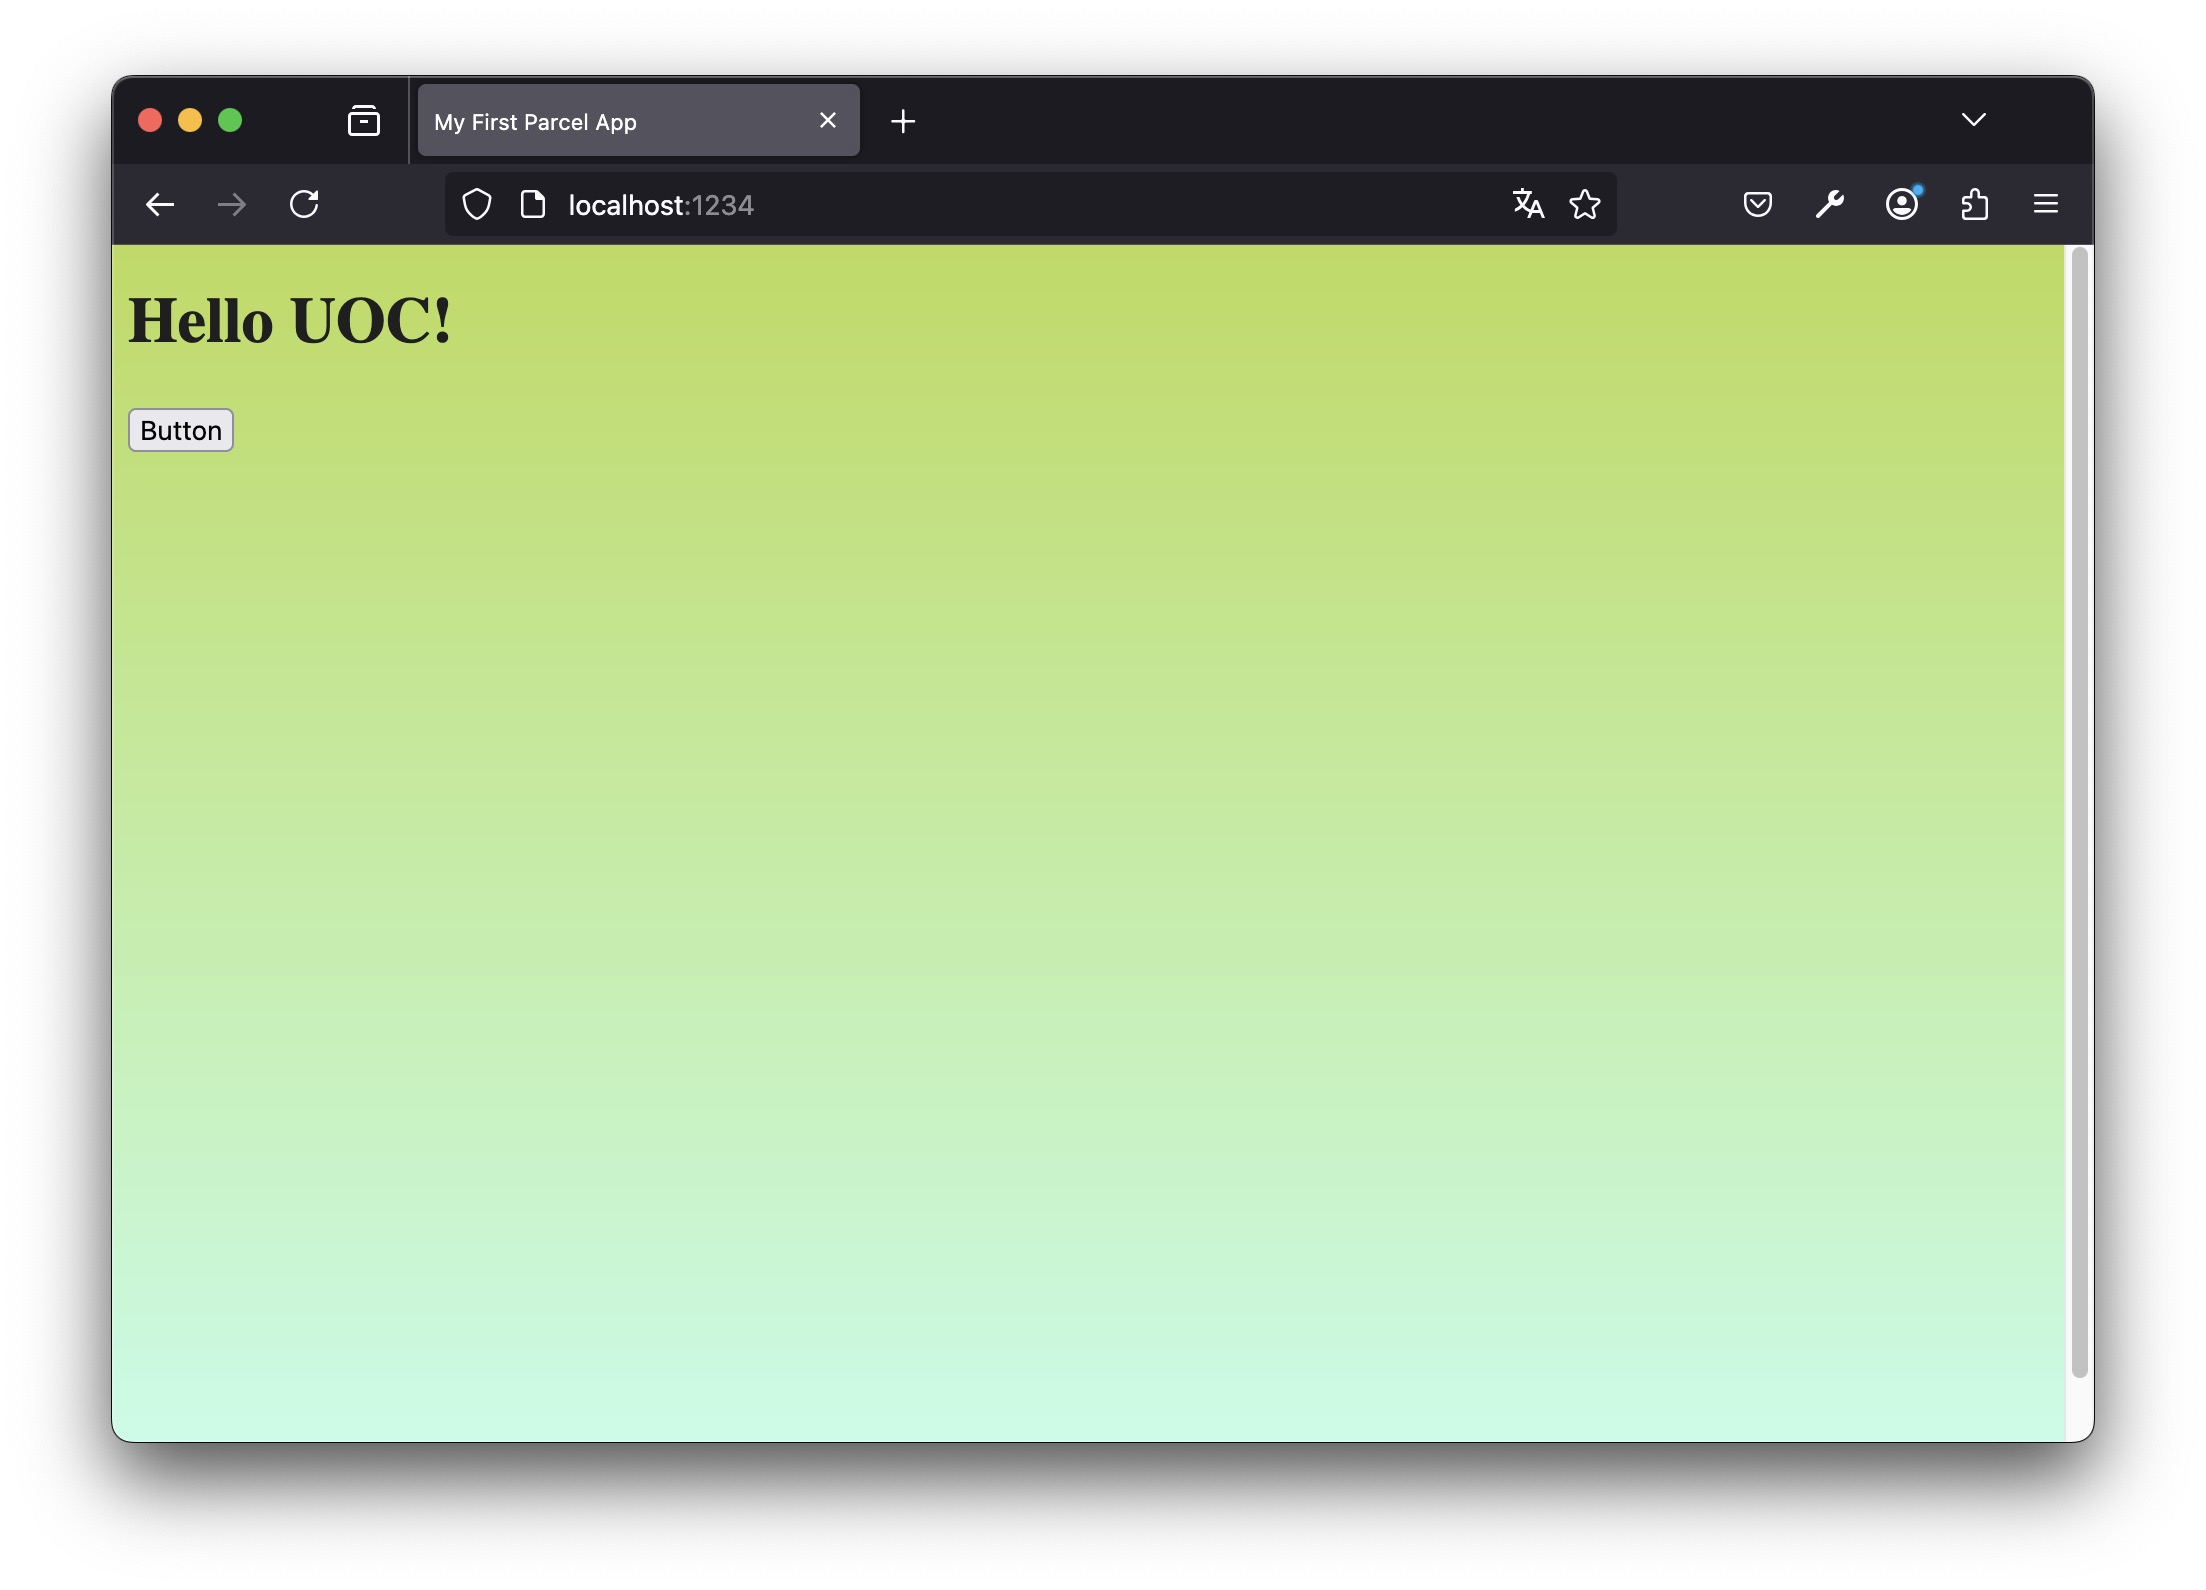
\includegraphics[width=0.8\textwidth]{./img/after-posthtml-include}
    \caption{Captura de pantalla del navegador con el botón renderizado correctamente}
    \label{fig:posthtml-include}
\end{figure}

\end{document}
